
\section{Introduction}

In this chapter, we will explore the BTCUSD(T) market across 5 major exchanges by following a visual approach on aggregated data. Our initial sampling approach will be across time (fixed time window). Key insights that will be extracted, will serve as the infrastructure of a dynamic way of sampling. 


\section{Volume}

It is commonly accepted that volume is one of the most important tools, for analyzing timeseries in finance. Exploring volume across exchanges is a significant task that will provide our analysis with the insights as to how someone should proceed in using trade-to-trade and aggregated volume in several windows, in order to create meaningful signals.

The trade data for BTCUSD begin as early as 2011, with few exchanges offering the opportunity to trade this asset. The first exchange was MtGox. It was launched in 2010 and shut down in April 2014 due to fraud, as more than 850,000 BTC were missing \cite{wiki_mt}. As time passed by, and BTC gained more traction, the trading volume upscaled significantly and more exchanges, such as Bitstamp, Kraken and Coinbase, appeared. Following 2017, a demographic shift took place: Institutions and retailers, started engaging with the crypto sphere and Bitcoin specifically in growing numbers \cite{med}. This was the period that Bitcoin become “known”.

\begin{figure}[h]
    \centering
    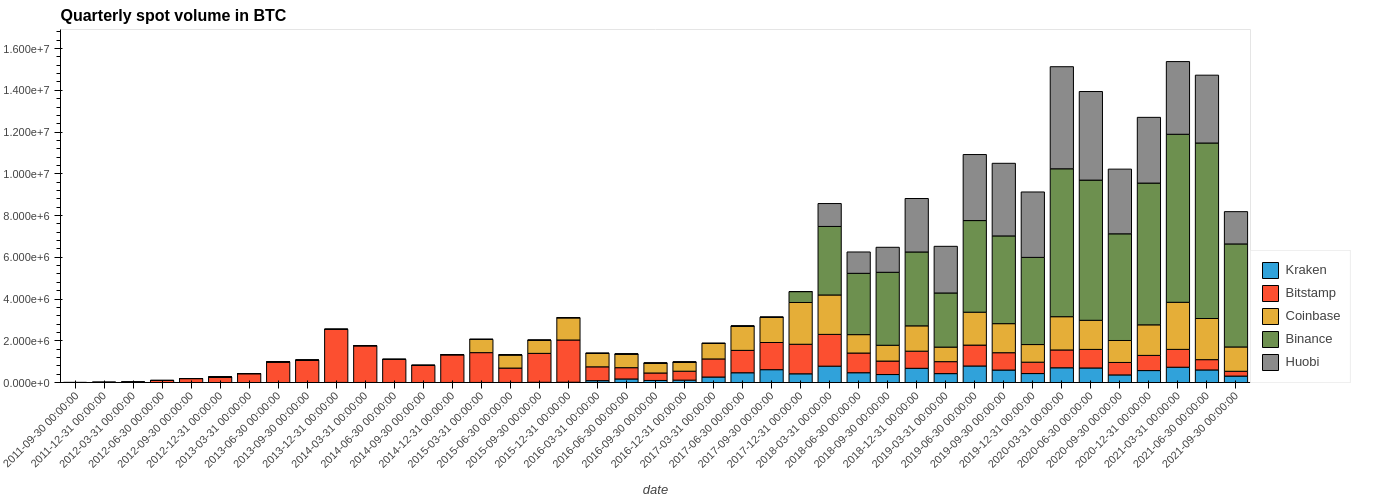
\includegraphics[width=10cm, height = 4cm]{historical_volume.png}
    \caption{Quarterly volume across spot exchanges.}
    \label{fig:hist_vol}
\end{figure}


As we can see in \ref{fig:hist_vol}, the overall trading volume begun to rise in early 2017, as more people were attracted to the impressive BTC bull run, up until that point. At this point, we could distinct the BTCUSD from BTCUSDT volume following the assumption that a retail trader is forced to use fiat currency in order to buy bitcoin for the first time, in some centralized exchange, thus the bitcoin volume on USD, could serve as an indicator of retail activity.


\begin{figure}[h]
    \centering
    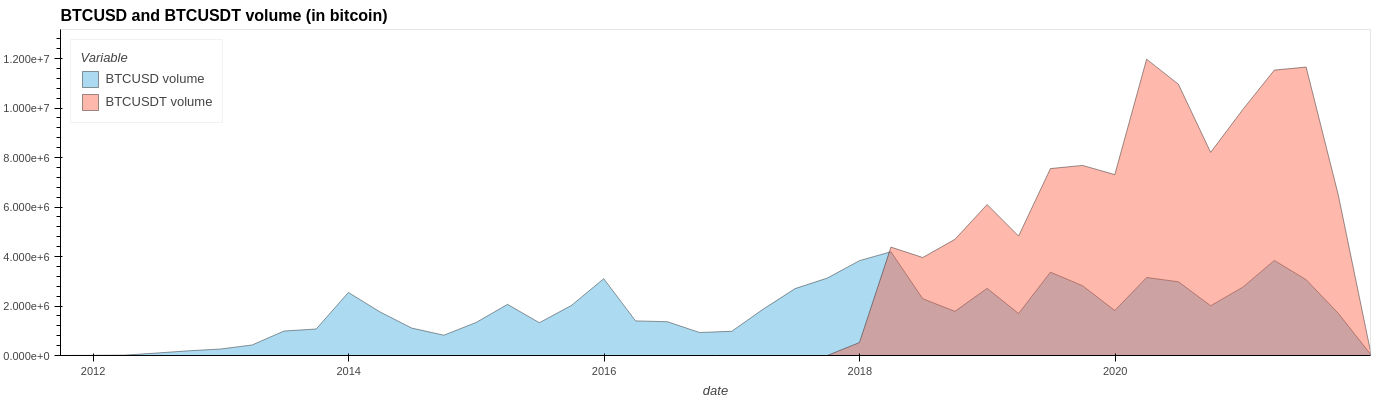
\includegraphics[width=10cm, height = 4cm]{volume2.png}
    \caption{BTCUSD and BTCUSDT spot trading volume (in bitcoin).}
    \label{fig:vol2}
\end{figure}

The first thing to notice in \ref{fig:vol2}, is that since the 2017 BTC bullrun, the BTCUSD volume (in bitcoin) is slightly elevated. Furthermore, since the introduction of USDT, the exchanges that offered BTCUSDT trading, easily surpassed those that offered only BTCUSD. The latter is to be expected, since USDT is 'tethered' to the USD (stable coin offering safety from volatility), while being at the same time easily transferable across exchanges in contrast to fiat. On the other hand, the \ref{fig:vol3} shows a steep increase in dollars traded that can be attributed to the increase in bitcoin price. 

\begin{figure}[h]
    \centering
    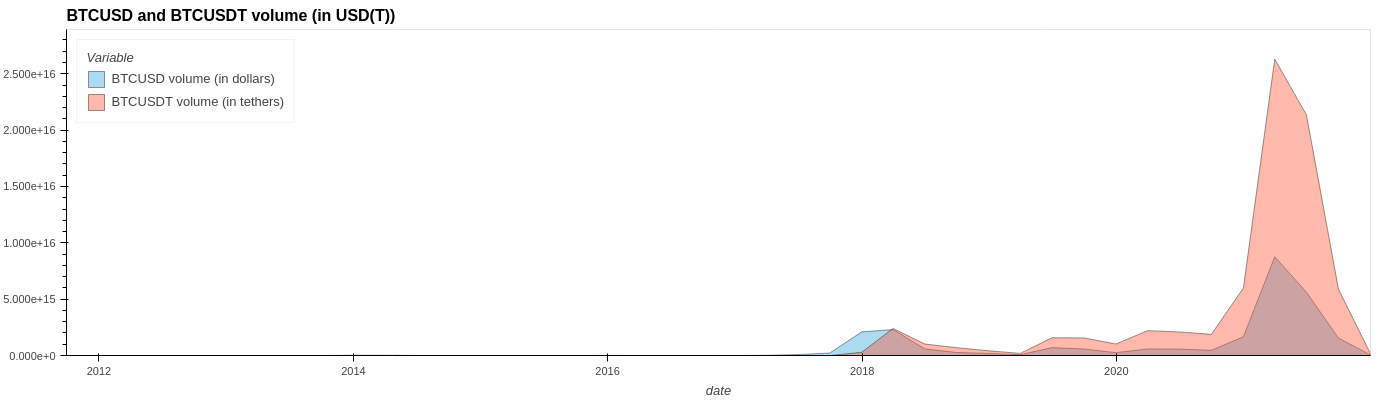
\includegraphics[width=10cm, height = 4cm]{usdusdt.png}
    \caption{BTCUSD and BTCUSDT spot trading volume (in USD(T)).}
    \label{fig:vol3}
\end{figure}

In the next four graphs \ref{fig:mean}, we can see the mean trading volume in bitcoin and dollars for BTCUSD and BTCUSDT. As we expect, in the upper two graphs, the mean trading volume decreases as bitcoin price increases. In contrast to the above, the bottom graphs, show an increase in mean trading volume, although, this increase, is different for the two markets: the BTCUSD market shows the 'anticipated' behavior that can be explained by the BTC price and the increased interest to this new asset, and the BTCUSDT market, exhibits a smaller increase in mean trading volume (dollars) even though the volume traded in USDT is higher than the volume traded in USD. The latter indicates the existence of many small buy/sell orders in the USDT markets.

\begin{figure}[H]
	\centering
    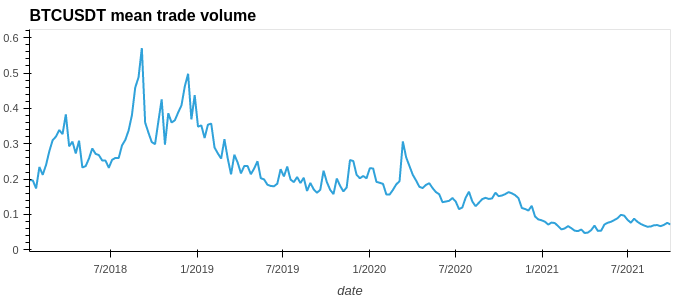
\includegraphics[width=6cm, height = 3.3cm]{mean1}
    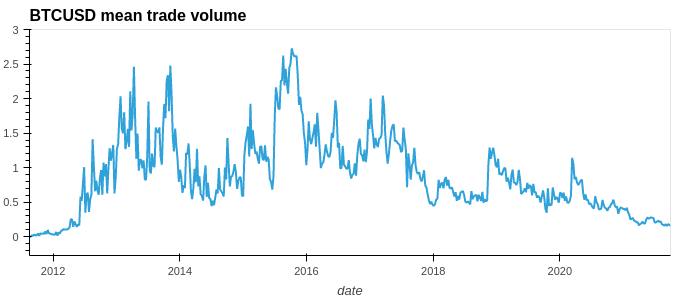
\includegraphics[width=6cm, height = 3.3cm]{mean2}
    \\[\smallskipamount]
    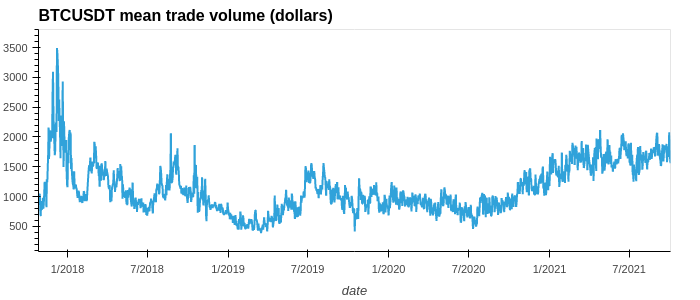
\includegraphics[width=6cm, height = 3.3cm]{mean3}
    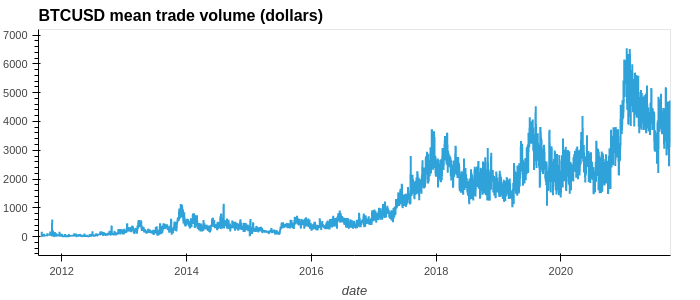
\includegraphics[width=6cm, height = 3.3cm]{mean4}
    \caption{Mean volume per trade.}
    \label{fig:mean}
\end{figure}


An approach that may disclose the “nature” of the investor based on the trade data at hand, would be to use the following framework of assumptions: 
\begin{itemize}
\item Retail traders are trading in integer dollar volumes, and
\item Institutional investors will more likely buy in OTC (Over The Counter) markets and sell in spot exchanges using sofisticated execution strategies.
\end{itemize} 

In order to extract the possible retail trades, an error of \( e = 0.05\$ \) was incorporated in creating two boundary conditions: 
\[ P - \texttt{int}(P) < e \text{ and },  P - \texttt{int}(P) > -e\] 
where \( P \) is the price in dollars at which a trade was executed. The role of the error \( e \), is to account for floating rounding errors \cite{app}.   

Furthermore, these trades could be made by a professional of a small magnitude and not a retail trader. For briefness purposes, we will refer to these trades, as retail trades, and the traders that initiated them, as retail traders. The above assumptions are flawed in the sense that someone can buy/sell in bitcoin denominated  values (0.5 btc or 1 btc), therefore, this metric can capture only a small percentage of retail trades. Nevertheless, based on the data that the authors possess, there is no other way to classify a trade as 'retail trade'.
 
In the figure \ref{fig:ret1}, we can see that the estimated number of retail trades on BTCUSDT, is from 4 to 12 times bigger than the one on BTCUSD. Since a retail trader that wishes to trade for the first time, is forced to use fiat currency, we could assume, that the BTCUSDT trades, were executed from retail traders that were active in previous market cycles as well (2017 bull run and before). 

On the top right graph, we can see the ratio of BTCUSDT to BTCUSD trades. We observe that the top is reached during May 2021, when the first large correction of the latest bull markets occured. 



\begin{figure}[H]
	\centering
    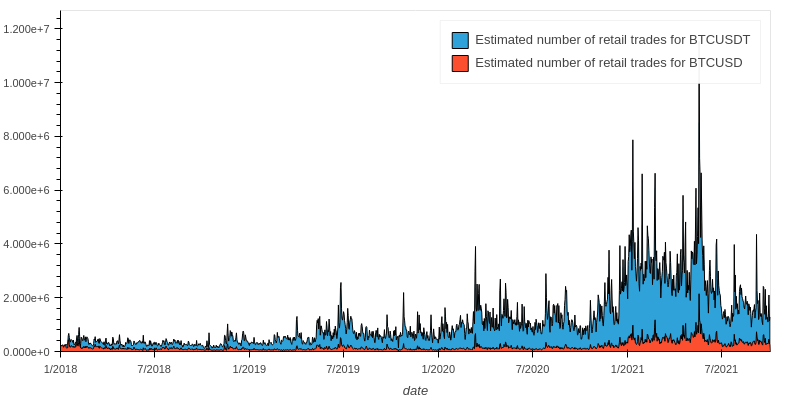
\includegraphics[width=6cm, height = 3.3cm]{ret_trades_1.png}
    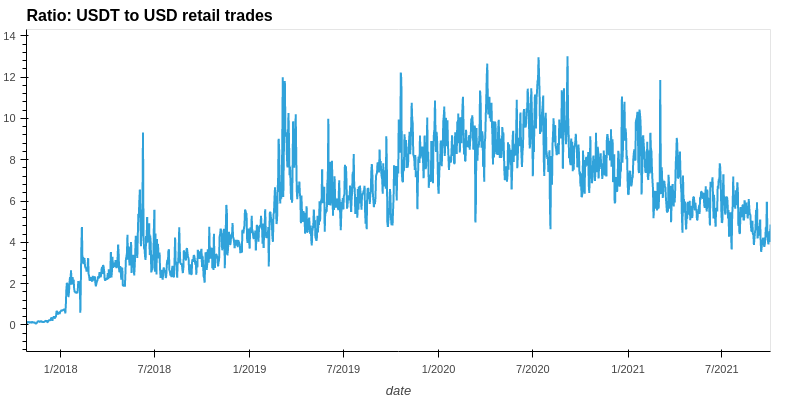
\includegraphics[width=6cm, height = 3.3cm]{ratio_ret_trades.png}
     \\[\smallskipamount]
    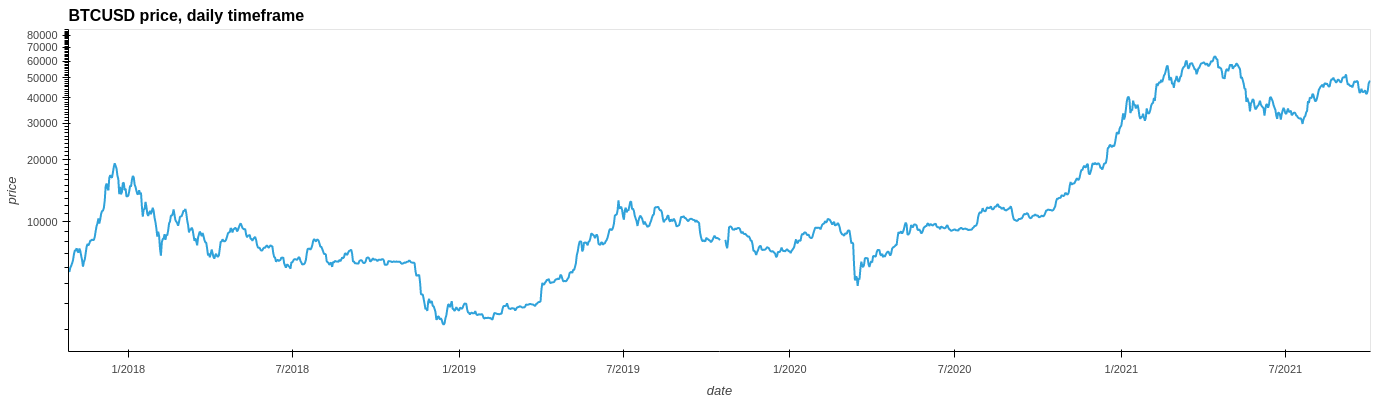
\includegraphics[width=12.2cm, height = 3.3cm]{price_retail.png}
	\caption{Retail trades and BTC price.}
    \label{fig:ret1}
\end{figure}

The increasing ratio indicates that BTCUSDT trades are relatively more precise in following the bull run (experienced retail traders) while the ratio starts declining, close to market top, indicating the timing when retail activity starts to gain traction in BTCUSD market, where is more likely for a 'first time retail trader' to trade.

On the next histograms, the difference in retail activity between BTCUSD and BTCUSDT becomes even more apparent. In the BTCUSD case, the graph is skewed to the left, with few days distributed to the extremes \( > 600,000 \). The BTCUSDT markets though, as indicated from standard deviation which is 3 times greater than the one in BTCUSD, show that the retail activity is distributed more evenly.

\begin{figure}[H]
	\centering
    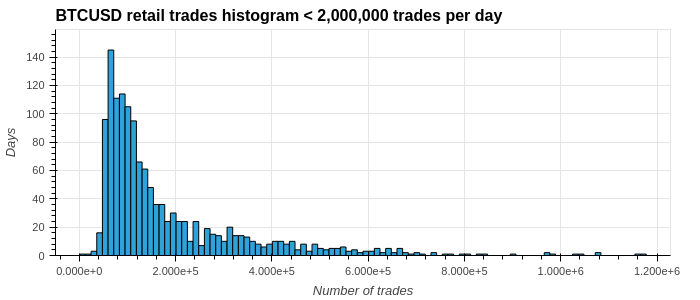
\includegraphics[width=6cm, height = 3.3cm]{btcusd_hist.png}
    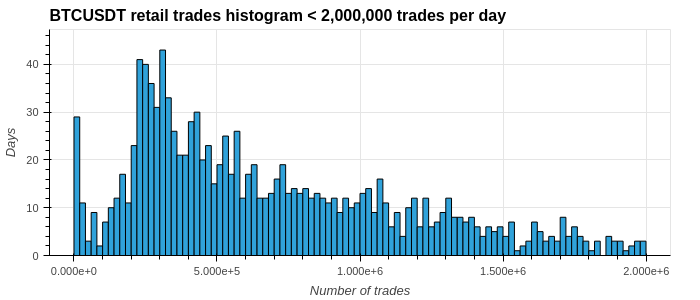
\includegraphics[width=6cm, height = 3.3cm]{btcusdt_hist.png}
    \caption{Histogram of BTCUSD and BTCUSDT no of retail trades per day}
    \label{fig:hist}
\end{figure}

From the summary statistics, we can see that the mean, 25\%, 50\% and 75\% are three to four times greater in BTCUSDT markets, indicative of the preference of retail traders to USDT.


\begin{center}
\begin{tabular}{ |p{3cm}||p{3cm}|p{3cm}| }
 \hline
 \multicolumn{3}{|c|}{Summary Statistics} \\
 \hline
  & BTCUSD  & BTCUSDT \\
 \hline
 count   & 1.372000e+03	   &1.206000e+03 \\
 mean &   1.837303e+05	  & 6.846854e+05   \\
 std &1.632955e+05 & 4.669768e+05\\
 min    &1.058000e+03 & 4.790000e+02\\
 25\% &   8.008925e+04  & 3.093760e+05\\
 50\% & 1.186430e+05  & 5.595545e+05   \\
 75\% & 2.206602e+05  & 9.985932e+05\\
 \hline
\end{tabular}
\end{center}


The differences between BTCUSD and BTCUSDT markets, extend to the bitcoin price as well. In the next figure \ref{fig:premium}, we can see that there are arbitrage opportunities between BTCUSD and BTCUSDT markets but not among the markets themselves. These opportunities seem to be available in periods of sudden price movements, and could be accredited to the difference in volume between the two markets. Throughout the 2021 bull market, there was a consistent discrepancy in the fiat premium index.


\begin{figure}[H]
	\centering
    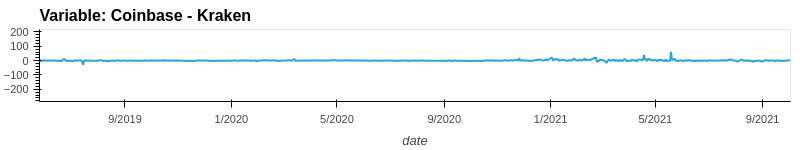
\includegraphics[width=12cm, height = 2.7cm]{pre1.png} \\
    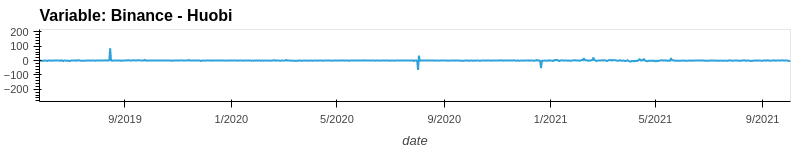
\includegraphics[width=12cm, height = 2.7cm]{pre2.png} \\
    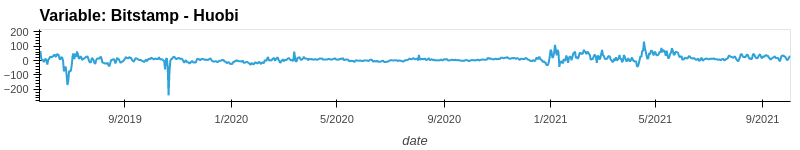
\includegraphics[width=12cm, height = 2.7cm]{pre3.png} \\
    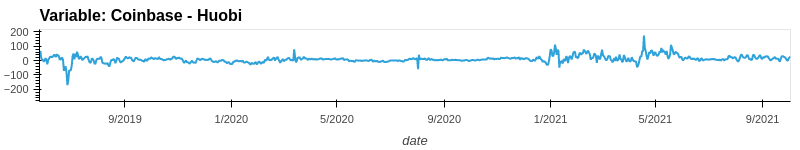
\includegraphics[width=12cm, height = 2.7cm]{pre4.png} \\
    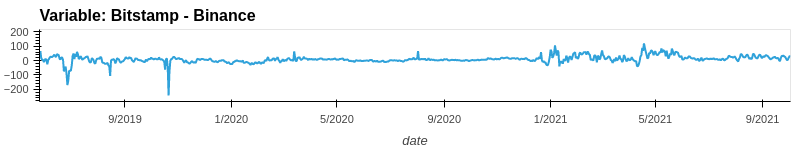
\includegraphics[width=12cm, height = 2.7cm]{pre5.png} \\
	\caption{Fiat premium.}
    \label{fig:premium}
\end{figure}


Such discrepancies could be a valuable source of imbalances, that should be useful for a more precise sampling. Next, we will explore volume, a bit deeper. We will decompose the covariance matrix of volume (eigen decomposition), of the BTCUSD
and BTCUSDT pairs. The computation will take place in a rolling fashion, under a fixed time interval, in order to capture the convergence of volume, between the exchanges and during different phases of the market.


\begin{figure}[H]
	\centering
    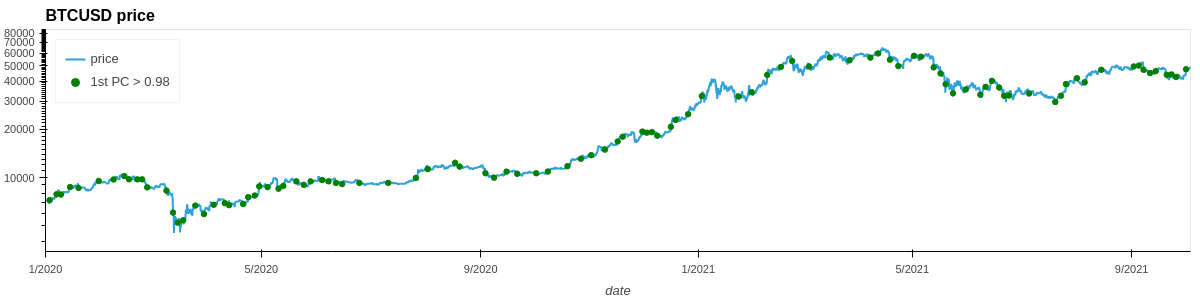
\includegraphics[width=12cm, height = 3cm]{cov1.png} \\
    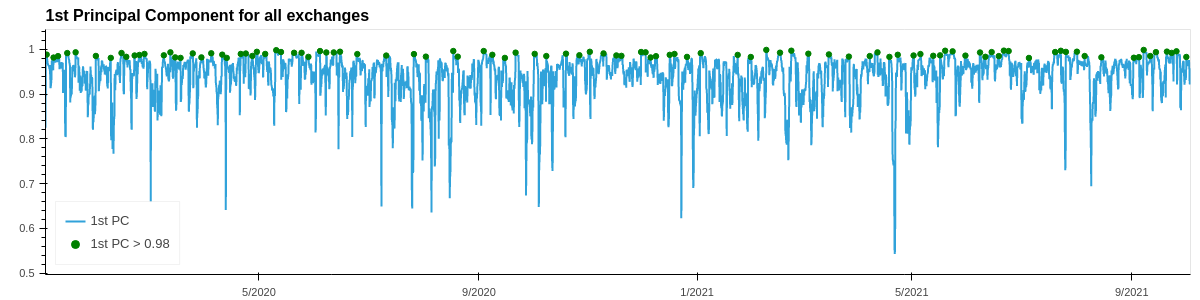
\includegraphics[width=12cm, height = 3cm]{cov2.png} \\
	\caption{PCA analysis - 1st principal component and BTCUSD price.}
    \label{fig:covmatrix}
\end{figure}

In the above figure \ref{fig:covmatrix}, we can see that based on the covariance of the volumes across exchanges, the 1st principal component seems to explain almost all variance, most of the time. This finding, enhances the idea that information is quickly transfered and volumes generally converge. The same must be tested for metrics other than covariance. An appropriate such metric, is the first principal component computed from the eigendecomposition of the Kendall correlation matrix. Since the volumes are not normally distributed (figure \ref{fig:kdevol}), we cannot use neither Pearson or Spearman correlation \cite{kendall}.


\begin{figure}[H]
	\centering
    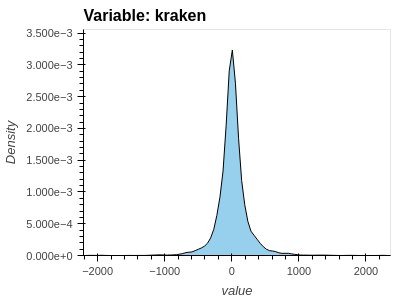
\includegraphics[width=4cm, height = 2.5cm]{kde1.png}
    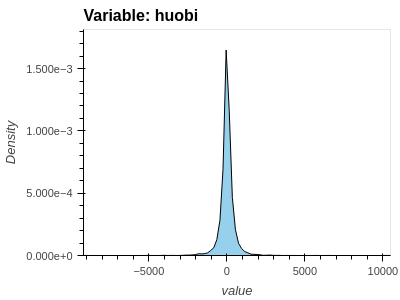
\includegraphics[width=4cm, height = 2.5cm]{kde2.png}
    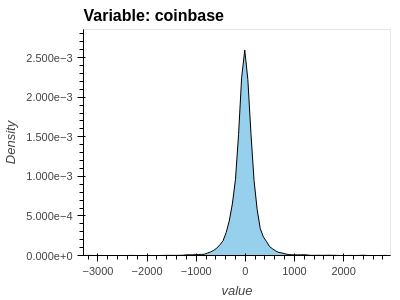
\includegraphics[width=4cm, height = 2.5cm]{kde3.png}
    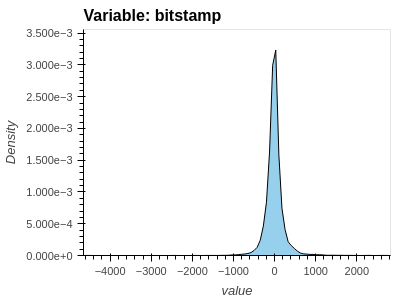
\includegraphics[width=4cm, height = 2.5cm]{kde4.png}
    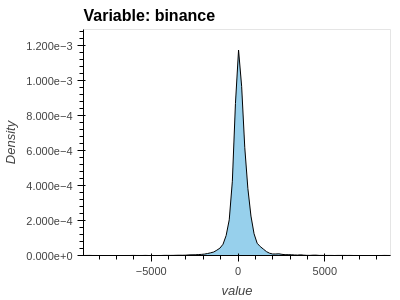
\includegraphics[width=4cm, height = 2.5cm]{kde5.png}
	\caption{KDE plot of volumes aggregated on 4h timeframe, for all exchanges.}
    \label{fig:kdevol}
\end{figure}


Kendall's Tau (\(\tau\)), is a non parametric test that is used to measure the correlation between two variables. There are three different variations of this test, but mostly the Tau-b (\(\tau_b\)) is used. The formula is:
\[
\tau_b = \frac{2(n_c - n_d)}{\sqrt{n(n-1) - G_x}\sqrt{n(n-1) - G_y}} 
\]

where:
\begin{itemize}
\item \(n_c\) is the number of concordant values
\item \(n_d\) is the number of discordant values
\item \(G_{x,y} = \sum{t_i(t_i-1)}\) where \(t_i\) is the number of tied values in the \(i\) group of the \(\{x,y\}\) variable
\end{itemize}

For the following graphs, we need to insert, the notion of positive and negative volumes. The notion of a positive volume (and negative accordingly) is the need to differentiate between the trading volume that leads to positive returns and volume in the market that lead to negative returns. The computations involved the sign of the returns \(b_t = sign\{p_t - p_{t-1}\}\), where \(p_t\) is the price at time \(t\) (this computation took place on tick data therefore \(t\) is the time measured in number of ticks), multiplied with volume at time \(t-1\) : \(b_t \cdot V_{t-1}\). Additionally, by classifying volumes, that inherit a positive or negative sign based on the returns, two sets are formed. 

\begin{figure}[H]
	\centering
    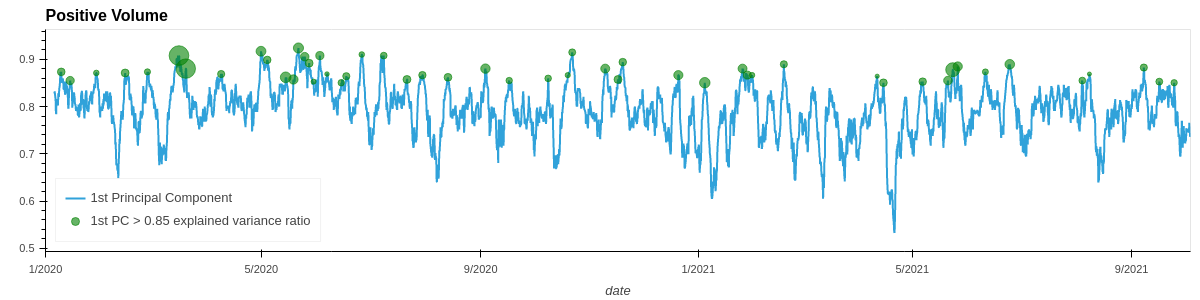
\includegraphics[width=12cm, height = 2.8cm]{kendal4.png} \\
    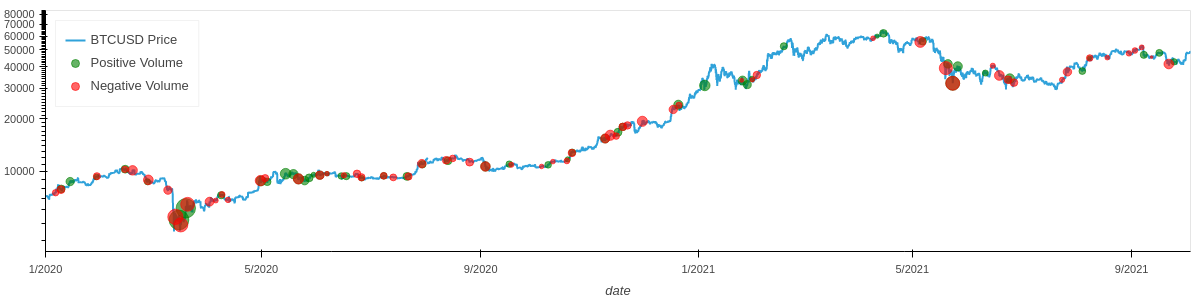
\includegraphics[width=12cm, height = 2.8cm]{kendal3.png} \\ 
    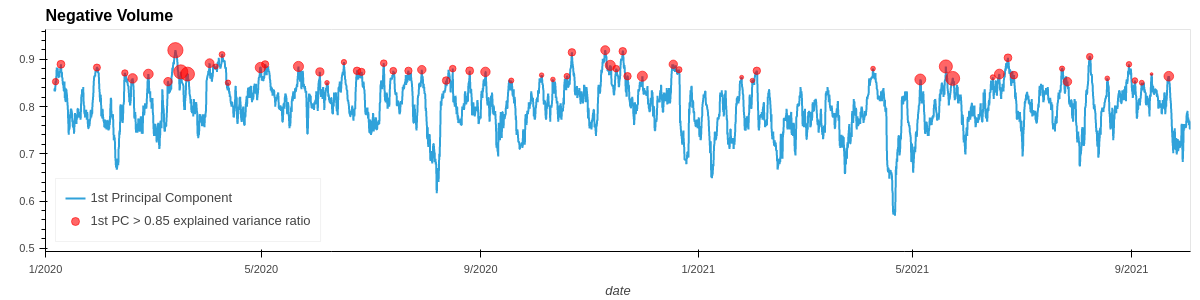
\includegraphics[width=12cm, height = 2.8cm]{kendal1.png} \\
    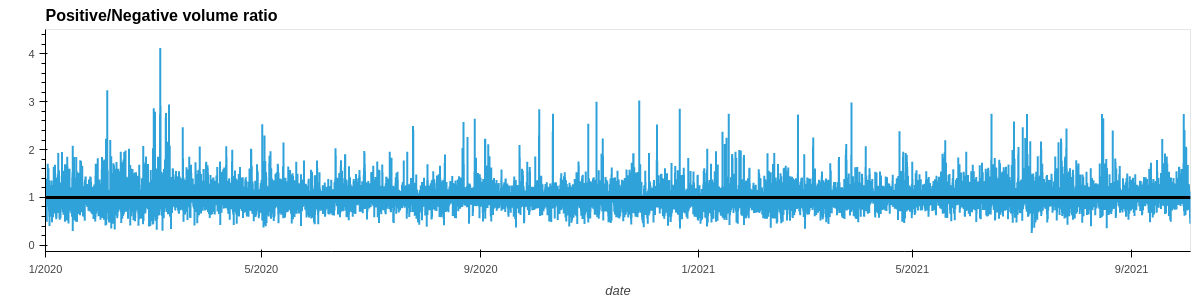
\includegraphics[width=12cm, height = 2.8cm]{kendal2.png} \\
	\caption{Eigendecomposition on kendal correlation matrix for positive and negative volume for \textbf{BTCUSDT} markets.}
    \label{fig:pcakendall}
\end{figure}

In figure \ref{fig:pcakendall} we can see the convergence of positive and negative volumes among BTCUSDT market. The 1st principal component has consistenly high explained variance ratio \( > 0.7 \) which shows that volume between Binance and Huobi, are following the same direction most of the time.

Upon close inspection, it seems that sudden price moves can be associated with higher convergence of volume between the BTCUSDT exchanges. The same seems to be the case, for all exchanges as well (figure \ref{fig:covmatrix}). That leads us to the idea that we could sample when there is convergence in a feature of choice (volume, positive-negative volume, buy/sell volume, number of trades per interval), assuming that in order for such an event to occur, there must be some new information. 

Next, we visualize the number of trades that take place in each exchange. In the figure \ref{fig:nooftrades}, we can see the number of trades aggregated in daily timeframe with the upper chard being in logarithmic scale. We observe that the USDT market is processing many more trades than the USD market. By calculating and comparing the mean number of trades per exchange across 2020 and 2021, we find that the mean trades per day of Binance is 5.5 time the mean of Coinbase, 32 times the mean of Kraken and approximately 37 times the mean of Bitstamp. We also observe that the number of trades (aggregated) is presented in waves, with visible spikes around significant price action. Again, these spikes, converge across all exchanges.  

\begin{figure}[H]
	\centering
    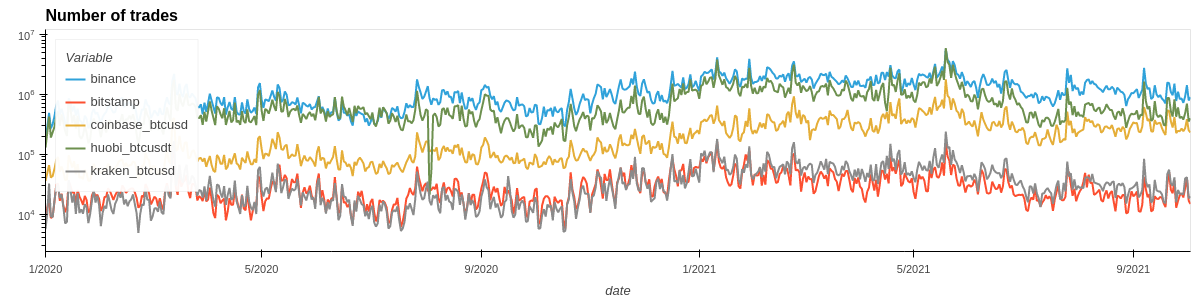
\includegraphics[width=12cm, height = 2.8cm]{No_of_trades_all2.png} \\
    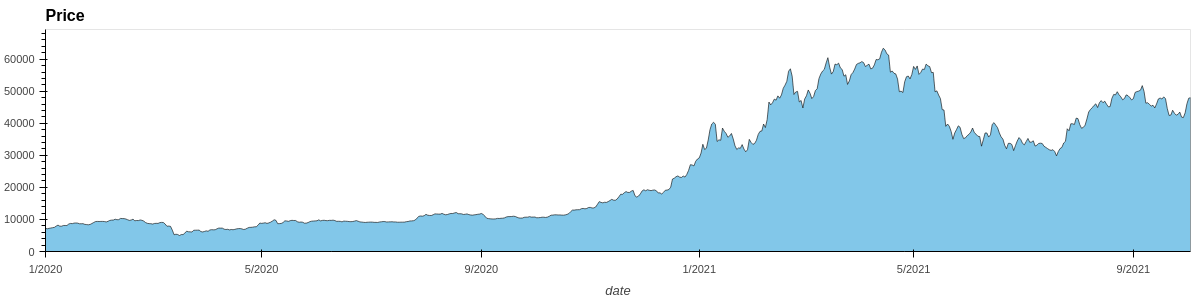
\includegraphics[width=12cm, height = 2.8cm]{No_of_trades_all1.png} \\ 
	\caption{The number of trades aggregated daily, for each exchange. Note that the upper chart is logarithmic.}
    \label{fig:nooftrades}
\end{figure}

In the next figure \ref{fig:nooftrades2}, we are separating the bid, from the offer trades, depending on who initiated each trade(based on  dataset labels buy-sell). First thing to notice is that our data is corrupted, since for approximately 15 days, all trades are classified as trades, initiated by buyers. Due to this shortcoming, in any attempt to use the side of the trade (bid-offer), we will have to exclude this portion of the dataset. Furthermore, the Binance, as expected, processes the largest amount of orders, either buying or selling, but in several spikes, Huobi seems to catch or even suprass Binance. Last but not least, it is interesting that the amount of trades in Coinbase's BTCUSD pair, are steadily increasing, catching up those of the BTCUSDT market.

\begin{figure}[H]
	\centering
    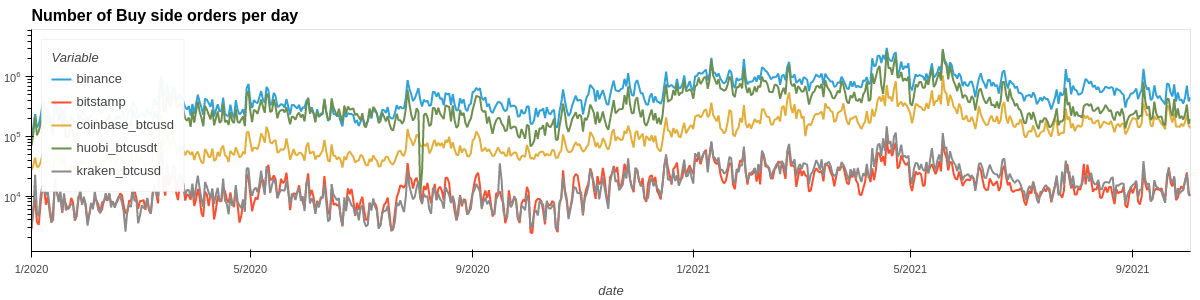
\includegraphics[width=12cm, height = 2.8cm]{nosell1.png} \\
    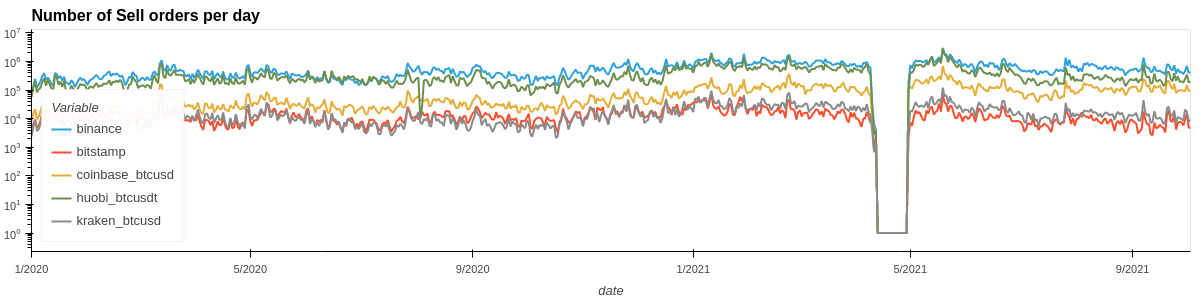
\includegraphics[width=12cm, height = 2.8cm]{nosell2.png} \\ 
	\caption{The number of buy and sell trades aggregated daily, for each exchange. Both charts are logarithmic.}
    \label{fig:nooftrades2}
\end{figure}


The next upper graph \ref{fig:cum}, is produced by taking the cumulative sums of buy side and sell side orders across all exchanges, and subtracting one from the other: 
\[ \text{cumsum}\{\text{Vol}_{\text{Buying}} - \text{Vol}_{\text{Selling}}\} \]
Just before the major bull run of 2020-2021, the selling volume, by far surpassed the buying volume, indicative of the uncertainty of that period (Covid19). Around October 2020, the cumulative sell volume peaked, as shown in the minimum of the graph. From then and on, the buy volume was steadily increasing, which coincides with the price action, at the beginning of the 2020-2021 bull run.  

The second graph is produced by taking the cumsum of the difference of buy and sell volume, but for each exchange individually. An interesting finding is that coinbase and bitstamp are processing more buy side volume than sell side, and more buy volume than any other exchange. The exact opposite is true for Binance, where sell volume is the highest. That alligns with our prior findings, in that BTCUSD market is the entrance of the 'first time' bitcoin buyer, who is attracted during the bull run. 


\begin{figure}[H]
	\centering
    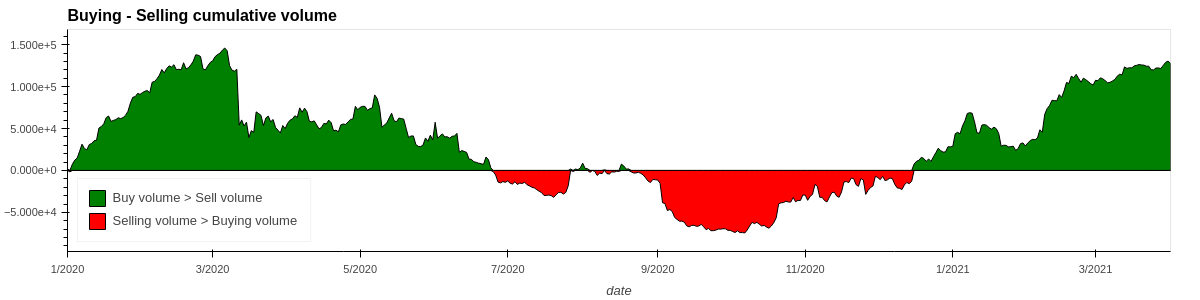
\includegraphics[width=12cm, height = 2.8cm]{buy-sell.png} \\
    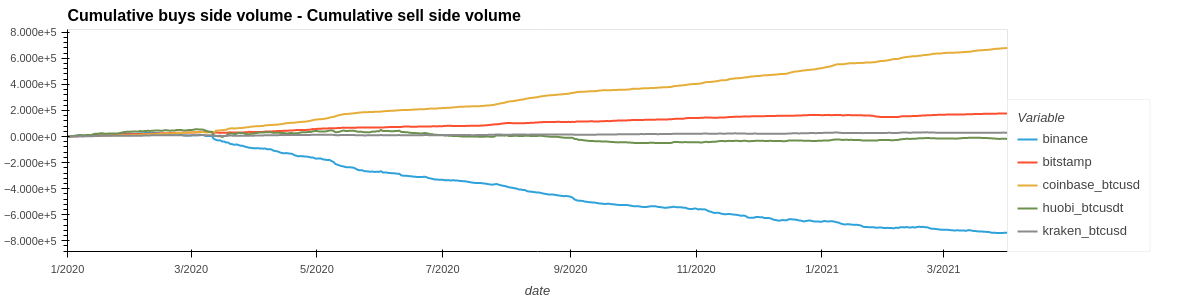
\includegraphics[width=12cm, height = 2.8cm]{cumdif.png} \\ 
	\caption{The number of buy and sell trades aggregated daily, for each exchange. Both charts are logarithmic.}
    \label{fig:cum}
\end{figure}


This discrepancy makes it clear, that even though each exchange has its own pool of
trades, the market dynamics are such, that one needs to consider each exchange not
only individually, but as a single identity as well with a unified liquidity pool. It appears from data, that it is possible that a single exchange can at times attract buyers and on the other hand, another one can attract sellers.
Such a behavior, can be explained by the simplicity of 
transferring tokens between exchanges (e.g. for arbitrage reasons). Especially USDT, XRP,
XLM and DOGE amongst others, seem to have viable liquidity, and very low
transaction finality times and fees. Coins such these, are prime candidates for transferring value fast and cheap.